% Options for packages loaded elsewhere
\PassOptionsToPackage{unicode}{hyperref}
\PassOptionsToPackage{hyphens}{url}
%
\documentclass[
]{article}
\usepackage{amsmath,amssymb}
\usepackage{lmodern}
\usepackage{iftex}
\ifPDFTeX
  \usepackage[T1]{fontenc}
  \usepackage[utf8]{inputenc}
  \usepackage{textcomp} % provide euro and other symbols
\else % if luatex or xetex
  \usepackage{unicode-math}
  \defaultfontfeatures{Scale=MatchLowercase}
  \defaultfontfeatures[\rmfamily]{Ligatures=TeX,Scale=1}
\fi
% Use upquote if available, for straight quotes in verbatim environments
\IfFileExists{upquote.sty}{\usepackage{upquote}}{}
\IfFileExists{microtype.sty}{% use microtype if available
  \usepackage[]{microtype}
  \UseMicrotypeSet[protrusion]{basicmath} % disable protrusion for tt fonts
}{}
\makeatletter
\@ifundefined{KOMAClassName}{% if non-KOMA class
  \IfFileExists{parskip.sty}{%
    \usepackage{parskip}
  }{% else
    \setlength{\parindent}{0pt}
    \setlength{\parskip}{6pt plus 2pt minus 1pt}}
}{% if KOMA class
  \KOMAoptions{parskip=half}}
\makeatother
\usepackage{xcolor}
\usepackage[margin=1in]{geometry}
\usepackage{color}
\usepackage{fancyvrb}
\newcommand{\VerbBar}{|}
\newcommand{\VERB}{\Verb[commandchars=\\\{\}]}
\DefineVerbatimEnvironment{Highlighting}{Verbatim}{commandchars=\\\{\}}
% Add ',fontsize=\small' for more characters per line
\usepackage{framed}
\definecolor{shadecolor}{RGB}{248,248,248}
\newenvironment{Shaded}{\begin{snugshade}}{\end{snugshade}}
\newcommand{\AlertTok}[1]{\textcolor[rgb]{0.94,0.16,0.16}{#1}}
\newcommand{\AnnotationTok}[1]{\textcolor[rgb]{0.56,0.35,0.01}{\textbf{\textit{#1}}}}
\newcommand{\AttributeTok}[1]{\textcolor[rgb]{0.77,0.63,0.00}{#1}}
\newcommand{\BaseNTok}[1]{\textcolor[rgb]{0.00,0.00,0.81}{#1}}
\newcommand{\BuiltInTok}[1]{#1}
\newcommand{\CharTok}[1]{\textcolor[rgb]{0.31,0.60,0.02}{#1}}
\newcommand{\CommentTok}[1]{\textcolor[rgb]{0.56,0.35,0.01}{\textit{#1}}}
\newcommand{\CommentVarTok}[1]{\textcolor[rgb]{0.56,0.35,0.01}{\textbf{\textit{#1}}}}
\newcommand{\ConstantTok}[1]{\textcolor[rgb]{0.00,0.00,0.00}{#1}}
\newcommand{\ControlFlowTok}[1]{\textcolor[rgb]{0.13,0.29,0.53}{\textbf{#1}}}
\newcommand{\DataTypeTok}[1]{\textcolor[rgb]{0.13,0.29,0.53}{#1}}
\newcommand{\DecValTok}[1]{\textcolor[rgb]{0.00,0.00,0.81}{#1}}
\newcommand{\DocumentationTok}[1]{\textcolor[rgb]{0.56,0.35,0.01}{\textbf{\textit{#1}}}}
\newcommand{\ErrorTok}[1]{\textcolor[rgb]{0.64,0.00,0.00}{\textbf{#1}}}
\newcommand{\ExtensionTok}[1]{#1}
\newcommand{\FloatTok}[1]{\textcolor[rgb]{0.00,0.00,0.81}{#1}}
\newcommand{\FunctionTok}[1]{\textcolor[rgb]{0.00,0.00,0.00}{#1}}
\newcommand{\ImportTok}[1]{#1}
\newcommand{\InformationTok}[1]{\textcolor[rgb]{0.56,0.35,0.01}{\textbf{\textit{#1}}}}
\newcommand{\KeywordTok}[1]{\textcolor[rgb]{0.13,0.29,0.53}{\textbf{#1}}}
\newcommand{\NormalTok}[1]{#1}
\newcommand{\OperatorTok}[1]{\textcolor[rgb]{0.81,0.36,0.00}{\textbf{#1}}}
\newcommand{\OtherTok}[1]{\textcolor[rgb]{0.56,0.35,0.01}{#1}}
\newcommand{\PreprocessorTok}[1]{\textcolor[rgb]{0.56,0.35,0.01}{\textit{#1}}}
\newcommand{\RegionMarkerTok}[1]{#1}
\newcommand{\SpecialCharTok}[1]{\textcolor[rgb]{0.00,0.00,0.00}{#1}}
\newcommand{\SpecialStringTok}[1]{\textcolor[rgb]{0.31,0.60,0.02}{#1}}
\newcommand{\StringTok}[1]{\textcolor[rgb]{0.31,0.60,0.02}{#1}}
\newcommand{\VariableTok}[1]{\textcolor[rgb]{0.00,0.00,0.00}{#1}}
\newcommand{\VerbatimStringTok}[1]{\textcolor[rgb]{0.31,0.60,0.02}{#1}}
\newcommand{\WarningTok}[1]{\textcolor[rgb]{0.56,0.35,0.01}{\textbf{\textit{#1}}}}
\usepackage{graphicx}
\makeatletter
\def\maxwidth{\ifdim\Gin@nat@width>\linewidth\linewidth\else\Gin@nat@width\fi}
\def\maxheight{\ifdim\Gin@nat@height>\textheight\textheight\else\Gin@nat@height\fi}
\makeatother
% Scale images if necessary, so that they will not overflow the page
% margins by default, and it is still possible to overwrite the defaults
% using explicit options in \includegraphics[width, height, ...]{}
\setkeys{Gin}{width=\maxwidth,height=\maxheight,keepaspectratio}
% Set default figure placement to htbp
\makeatletter
\def\fps@figure{htbp}
\makeatother
\setlength{\emergencystretch}{3em} % prevent overfull lines
\providecommand{\tightlist}{%
  \setlength{\itemsep}{0pt}\setlength{\parskip}{0pt}}
\setcounter{secnumdepth}{-\maxdimen} % remove section numbering
\ifLuaTeX
  \usepackage{selnolig}  % disable illegal ligatures
\fi
\IfFileExists{bookmark.sty}{\usepackage{bookmark}}{\usepackage{hyperref}}
\IfFileExists{xurl.sty}{\usepackage{xurl}}{} % add URL line breaks if available
\urlstyle{same} % disable monospaced font for URLs
\hypersetup{
  pdftitle={Homework Assignment \#2},
  pdfauthor={Math 437 - Modern Data Analysis},
  hidelinks,
  pdfcreator={LaTeX via pandoc}}

\title{Homework Assignment \#2}
\author{Math 437 - Modern Data Analysis}
\date{Due February 24, 2023}

\begin{document}
\maketitle

\begin{Shaded}
\begin{Highlighting}[]
\FunctionTok{library}\NormalTok{(tidyverse)}
\end{Highlighting}
\end{Shaded}

\begin{verbatim}
## -- Attaching core tidyverse packages ------------------------ tidyverse 2.0.0 --
## v dplyr     1.1.0     v readr     2.1.4
## v forcats   1.0.0     v stringr   1.5.0
## v ggplot2   3.4.1     v tibble    3.2.0
## v lubridate 1.9.2     v tidyr     1.3.0
## v purrr     1.0.1     
## -- Conflicts ------------------------------------------ tidyverse_conflicts() --
## x dplyr::filter() masks stats::filter()
## x dplyr::lag()    masks stats::lag()
## i Use the ]8;;http://conflicted.r-lib.org/conflicted package]8;; to force all conflicts to become errors
\end{verbatim}

\begin{Shaded}
\begin{Highlighting}[]
\FunctionTok{library}\NormalTok{(dplyr)}
\FunctionTok{library}\NormalTok{(ggplot2)}
\FunctionTok{library}\NormalTok{(ISLR2)}
\FunctionTok{library}\NormalTok{(DescTools)}
\end{Highlighting}
\end{Shaded}

\hypertarget{instructions}{%
\section{Instructions}\label{instructions}}

You should submit either two or three files:

\begin{enumerate}
\def\labelenumi{\arabic{enumi}.}
\tightlist
\item
  You should write your solutions to the Simulation and Applied Problems
  in this R Markdown file and submit the (.Rmd) file.
\item
  You should knit the final solution file to pdf and submit the pdf. If
  you are having trouble getting code chunks to run, add
  \texttt{eval\ =\ FALSE} to the chunks that do not run. If you are
  having trouble getting R Studio to play nice with your LaTeX
  distribution, I will begrudgingly accept an HTML file instead.
\item
  Solutions to the Key Terms and Conceptual Problems can be submitted in
  a separate Word or pdf file or included in the same files as your
  solutions to the Simulation and Applied Problems.
\end{enumerate}

This homework assignment is worth a total of \textbf{40 points}.

\hypertarget{key-terms-5-pts}{%
\section{Key Terms (5 pts)}\label{key-terms-5-pts}}

Read Chapter 13 of Introduction to Statistical Learning, Second Edition.
Based on your reading, answer the following questions.

\begin{enumerate}
\def\labelenumi{\arabic{enumi}.}
\tightlist
\item
  What is a \emph{p-value}? What is the difference between a one-sided
  and a two-sided p-value?
\end{enumerate}

Answer: The p-value is the probability of observing a test statistic
that is equal to or more extreme than the observed statistic under the
assumption that \(H_0\) is true. The difference between the one and two
sided p-value is a two sided p-value is based on the absolute value of
the test statistic, i.e.~our t-score could be 1.65 or -1.65 but the one
sided p-value is only looking at one of those values.

\begin{enumerate}
\def\labelenumi{\arabic{enumi}.}
\setcounter{enumi}{1}
\tightlist
\item
  In traditional NHST-style significance testing, what are the two
  possible decisions? When do we make each decision?
\end{enumerate}

Answer: The two possible decisions are to reject the null hypothesis,
occurs when our p-value is less than our pre-determined alpha. The other
is to fail to reject our null hypothesis which occurs when our p-value
is larger than that alpha.

\begin{enumerate}
\def\labelenumi{\arabic{enumi}.}
\setcounter{enumi}{2}
\tightlist
\item
  What is the difference between a \emph{Type I Error} and a \emph{Type
  II Error}?
\end{enumerate}

Answer: The best case of Type I and Type II error I have learned is the
story of the boy who cried wolf. At first the city makes a Type I error
by rejecting \(H_0\) (there is no wolf) when in fact there was no wolf,
followed by them making a Type II error by not rejecting \(H_0\) (again
there is no wolf) when in reality there is. So a Type I Error occurs
when we reject \(H_0\) when \(H_0\) was in fact true and a Type II Error
is occurs when we do not reject \(H_0\) when \(H_a\) was true.

\begin{enumerate}
\def\labelenumi{\arabic{enumi}.}
\setcounter{enumi}{3}
\item
  Briefly explain why it is necessary to adjust the significance level
  (or equivalently, the p-values) when testing a large number of null
  hypotheses. Answer: The reason why we need to adjust the significance
  level when testing a large number of null hypotheses is to account for
  the chance of seeing a small p-value strictly by chance. When a large
  number of tests are conducted, the number of Type I Errors we expect
  to make will increase so it becomes necessary to adjust the
  significance level to control for this.
\item
  Compare and contrast the \emph{Family-Wise Error Rate} (FWER) and the
  \emph{False Discovery Rate} (FDR). Answer: The FWER and FDR are
  similar in the sense that both are looking at the likelihood of Type I
  Error rates are but are very different in ideas. FWER looks at the
  probability of making at least one Type I Error across \(m\) tests
  whereas FDR is looking to minimize the proportion of type one error
  rates and total rejections of \(H_0\).
\item
  Compare and contrast the \emph{Bonferroni Method} and \emph{Holm's
  Step-Down Method} for controlling the FWER. Answer: Bonferroni \&
  Holm's Step-Down Method both aim to decrease (or control) the FWER
  based on the number of tests conducted without making assumptions
  about the form of \(H_0\), the choice of test statistic, or the
  (in)dependence of p-values. Bonferroni's method adjusts the
  significance level based purely on the number of tests conducted,
  \(m\), so that our new significance level is
  \(\alpha^* = \frac{\alpha}{m}\). Holm's Step-Down Method ranks the
  p-values from every test in ascending order and begins comparing them
  beginning with the most conservative significance level of
  \(\alpha^* = \frac{\alpha}{m}\) for the smallest p-value and if the
  p-value is significant, it adjusts the significance level for the
  subsequent p-value to be \(\alpha^* = \frac{\alpha}{m - 1}\) and so on
  until a non-significant p-value is found, resulting in a higher number
  of null hypotheses rejected.
\item
  Why do we prefer to use \emph{Tukey's Method} or \emph{Scheffe's
  Method} to control the FWER? In what conditions is it appropriate to
  use those methods instead of the Bonferroni or Holm methods?
\end{enumerate}

Answer: We prefer to use Tukey's or Scheffe's Method because they allows
us to further control the FWER while increasing power. It is more
appropriate to use Tukeys methods when we have dependence between
p-values caused by similar hypotheses tests so we can conduct pairwise
comparisons and we can use Scheffe's to control FWER at a specific
significance level \(\alpha\).

\begin{enumerate}
\def\labelenumi{\arabic{enumi}.}
\setcounter{enumi}{7}
\item
  Briefly describe the \emph{Benjamini-Hochberg} procedure for
  controlling the FDR. Answer: The Benjamini-Hochberg procedure begins
  by deciding on a specific q value to control the FDR at. Then finding
  and ordering our p-values such that the smallest p-value is first to
  the largest p-value. Next we define L as the maximum p-value for which
  the jth p-value is less than q(j/m). Lastly we reject all p-values for
  which p(j) is less than p(L).
\item
  What is/are the major assumption(s) of a \emph{permutation test}? What
  is the general procedure for obtaining the null distribution of a test
  statistic using a permutation test? Answer: The major assumptions of a
  permutation test is that the distribution of X and Y are similar such
  that values can be interchanged when calculating our T-values. The
  process of obtaining the null distribution is through permuting n(x) +
  n(y) B times for a large number, B. Once that is done the distribution
  of B is that null distribution.
\item
  When is it useful/recommended to use a permutation testing approach as
  opposed to a traditional theory-based approach? Answer: We would want
  to use a permutation test when the distribution of our data does not
  follow a known shape. When our distribution follows that of a
  t-distribution, chi-squared distribution, F-distribution, etc. a
  traditional based approach works wonderful but when we are not
  following that we are inclined to go towards permutation methods.
\end{enumerate}

\hypertarget{conceptual-problems}{%
\section{Conceptual Problems}\label{conceptual-problems}}

\hypertarget{conceptual-problem-1-5-pts}{%
\subsection{Conceptual Problem 1 (5
pts)}\label{conceptual-problem-1-5-pts}}

Textbook Exercise 13.7.6:

For each of the three panels in Figure 13.3, answer the following
questions: (a) How many false positives, false negatives, true
positives, true negatives, Type I errors, and Type II errors result from
applying the Bonferroni procedure to control the FWER at level
\(\alpha = 0.05\)?

\begin{enumerate}
\def\labelenumi{\arabic{enumi}.}
\item
  Panel one has seven true positives, one false negative, and two true
  negatives. Thus it has One Type II Error and no Type I Errors.
\item
  Panel two has seven true positives, one false negative, and two true
  negatives. Thus it has one Type II Error and no Type I Errors.
\item
  Panel three has three true positives, five false negatives, and two
  true negatives. Thus it has five Type II Errors.
\end{enumerate}

\begin{enumerate}
\def\labelenumi{(\alph{enumi})}
\setcounter{enumi}{1}
\tightlist
\item
  How many false positives, false negatives, true positives, true
  negatives, Type I errors, and Type II errors result from applying the
  Holm procedure to control the FWER at level \(\alpha = 0.05\)?
\end{enumerate}

\begin{enumerate}
\def\labelenumi{\arabic{enumi}.}
\item
  Panel one has seven true positives, one false negative, and two true
  negatives. Thus it has One Type II Error and no Type I Errors.
\item
  Panel two has eight true positives, and two true negatives. Thus it
  has no Type I Errors or Type II Errors.
\item
  Panel two has eight true positives, and two true negatives. Thus it
  has no Type I Errors or Type II Errors.
\end{enumerate}

\begin{enumerate}
\def\labelenumi{(\alph{enumi})}
\setcounter{enumi}{2}
\tightlist
\item
  What is the false discovery rate associated with using the Bonferroni
  procedure to control the FWER at level \(\alpha = 0.05\)?
\end{enumerate}

The False discovery rate associated with using the Bonferroni procedure
to control the FWER at level \(\alpha = 0.05\) is 0 for all three panels
since there are no true null hypotheses being rejected.

\begin{enumerate}
\def\labelenumi{(\alph{enumi})}
\setcounter{enumi}{3}
\tightlist
\item
  What is the false discovery rate associated with using the Holm
  procedure to control the FWER at level \(\alpha = 0.05\)?
\end{enumerate}

The FDR associated with using the Holm procedure to control the FWER at
level \(\alpha = 0.05\) is 0 since there are no false positives.

\begin{enumerate}
\def\labelenumi{(\alph{enumi})}
\setcounter{enumi}{4}
\tightlist
\item
  How would the answers to (a) and (c) change if we instead used the
  Bonferroni procedure to control the FWER at level \(\alpha = 0.001\)?
\end{enumerate}

\begin{enumerate}
\def\labelenumi{\alph{enumi})}
\item
  At \(\alpha = 0.001\), both panel one and two would have three false
  negatives (Type II Errors), two true negatives, and five true
  positives. Panel three would have five false negatives (Type II
  Errors), two true negatives, and three true positives. No panel has
  false positives (Type I Errors).
\item
  The FDR would remain at 0 since there is still no false positives.
\end{enumerate}

\hypertarget{conceptual-problem-2-2-pts}{%
\subsection{Conceptual Problem 2 (2
pts)}\label{conceptual-problem-2-2-pts}}

Suppose that we test \(m = 1000\) independent null hypotheses, of which
10\% are true, at significance level \(\alpha = 0.05\) and achieve a
false discovery rate of \(q = 0.20\). Construct a table following Table
13.2 in the textbook, identifying the appropriate values of \(V\),
\(S\), \(U\), \(W\), and \(R\) in this situation. Answer:

\(m_0\) = 100

\(V = \alpha*m_0 = 5\)

\(0.2 = V/(V + S)\) -\textgreater{} \(S = 20\)

\[
\begin{tabular}{|c|c c|c|}  \hline
 & $H_0$ True & $H_0$ False & Total \\
\hline 
Reject $H_0$ & 5 & 20 & 25 \\ 
Do not reject $H_0$ & 95 & 880 & 975 \\ 
 \hline
Total & 100 & 900 & 1000 \\ 
\hline  
\end{tabular}
\]

\hypertarget{conceptual-problem-3-3-pts}{%
\subsection{Conceptual Problem 3 (3
pts)}\label{conceptual-problem-3-3-pts}}

Suppose that we test \(m = 1000\) independent null hypotheses, of which
an unknown number \(m_0\) are true, at significance level
\(\alpha = 0.05\). Suppose that each test also has a power of 0.80. Find
and plot the false discovery rate as a function of \(m_0\). Answer:

\begin{Shaded}
\begin{Highlighting}[]
\NormalTok{al }\OtherTok{=} \FloatTok{0.05}
\NormalTok{fdr }\OtherTok{=} \ControlFlowTok{function}\NormalTok{(m0)\{al}\SpecialCharTok{*}\NormalTok{m0}\SpecialCharTok{/}\NormalTok{(al}\SpecialCharTok{*}\NormalTok{m0 }\SpecialCharTok{+} \DecValTok{800} \SpecialCharTok{{-}} \FloatTok{0.8}\SpecialCharTok{*}\NormalTok{m0)\}}
\FunctionTok{plot}\NormalTok{(fdr, }\DecValTok{1}\NormalTok{, }\DecValTok{1000}\NormalTok{, }\AttributeTok{xlab =} \StringTok{"m\_0"}\NormalTok{, }\AttributeTok{ylab =} \StringTok{"False Discovery Rate"}\NormalTok{)}
\end{Highlighting}
\end{Shaded}

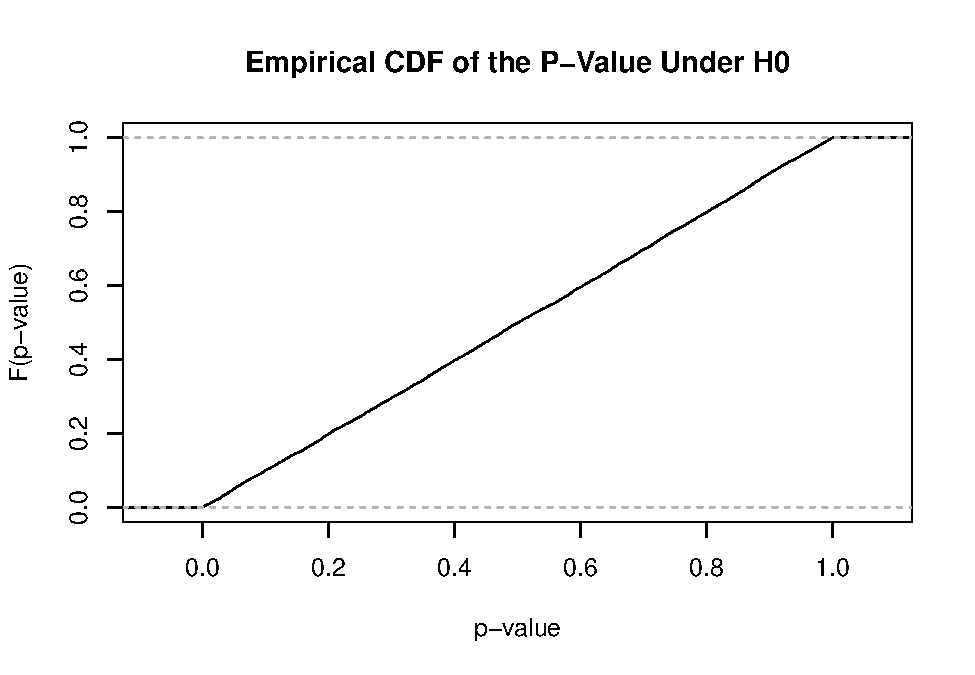
\includegraphics{Homework2_files/figure-latex/unnamed-chunk-3-1.pdf}

\hypertarget{conceptual-problem-4-2.5-pts}{%
\subsection{Conceptual Problem 4 (2.5
pts)}\label{conceptual-problem-4-2.5-pts}}

Textbook Exercise 5.4.2 parts (a), (b), and (c).:

We will now derive the probability that a given observation is part of a
bootstrap sample. Suppose that we obtain a bootstrap sample from a set
of n observations. (a) What is the probability that the first bootstrap
observation is not the jth observation from the original sample? Justify
your answer. Answer: The probability of the first bootstrap observation
not being the jth observation seems very likely. Thus logically the odds
of any one observation being the jth is 1/n, so the odds of it not being
the jth must then be 1 - 1/n.

\begin{enumerate}
\def\labelenumi{(\alph{enumi})}
\setcounter{enumi}{1}
\item
  What is the probability that the second bootstrap observation is not
  the jth observation from the original sample? Answer: Using the same
  logic as the previous problem the probability of the second
  observation being the jth observation is also 1/n.~Then the
  probability that it is not is also 1 - 1/n.
\item
  Argue that the probability that the jth observation is not in the
  bootstrap sample is (1 - 1/n)\^{}n.
\end{enumerate}

Answer: Since we are using a bootstrap sample the samples are then
independent. Meaning that the probability of jth observation not being
in the bootstrap sample is the same as the previous two questions but
all n times, thus the formula is (1-1/n)\^{}n

\hypertarget{simulation-problems}{%
\section{Simulation Problems}\label{simulation-problems}}

\hypertarget{simulation-problem-1-code-1-pt-explanation-0.5-pts}{%
\subsection{Simulation Problem 1 (Code: 1 pt; Explanation: 0.5
pts)}\label{simulation-problem-1-code-1-pt-explanation-0.5-pts}}

Textbook Exercise 5.4.2 parts (e), (g), and (h). For part (g), you
should create a line plot (using either \texttt{plot} with argument
\texttt{type\ =\ "l"} or \texttt{geom\_line}). Then, to make clearer
what you should be commenting on, find the limit as
\(n \rightarrow \infty\) of the probability that the \(j^{th}\)
observation is in your bootstrap sample and add a horizontal red line
(using \texttt{abline} or \texttt{geom\_hline}) at that value. (Hint:
the limit as \(n \rightarrow \infty\) of the expression in part (c) is
well-known and easily found on the Internet.)

\begin{enumerate}
\def\labelenumi{\alph{enumi})}
\setcounter{enumi}{4}
\item
  Using the formula in the previous question and plugging in 100, we can
  see our probability of the jth observation being in our bootstrap
  sample is 1-(1-(1/100))\^{}100 = 0.634
\item
\end{enumerate}

\begin{Shaded}
\begin{Highlighting}[]
\NormalTok{a }\OtherTok{=} \DecValTok{1}\SpecialCharTok{:}\DecValTok{10}
\NormalTok{b }\OtherTok{\textless{}{-}} \DecValTok{1}\SpecialCharTok{{-}}\NormalTok{(}\DecValTok{1}\SpecialCharTok{{-}}\NormalTok{(}\DecValTok{1}\SpecialCharTok{/}\NormalTok{a))}\SpecialCharTok{\^{}}\NormalTok{a}
\NormalTok{c }\OtherTok{=} \DecValTok{1}\SpecialCharTok{:}\DecValTok{100}
\NormalTok{d }\OtherTok{\textless{}{-}} \DecValTok{1}\SpecialCharTok{{-}}\NormalTok{(}\DecValTok{1}\SpecialCharTok{{-}}\NormalTok{(}\DecValTok{1}\SpecialCharTok{/}\NormalTok{c))}\SpecialCharTok{\^{}}\NormalTok{c}
\NormalTok{x }\OtherTok{=} \DecValTok{1}\SpecialCharTok{:}\DecValTok{10000}
\NormalTok{y }\OtherTok{\textless{}{-}} \DecValTok{1}\SpecialCharTok{{-}}\NormalTok{(}\DecValTok{1}\SpecialCharTok{{-}}\NormalTok{(}\DecValTok{1}\SpecialCharTok{/}\NormalTok{x))}\SpecialCharTok{\^{}}\NormalTok{x}


\FunctionTok{par}\NormalTok{(}\AttributeTok{mfrow=}\FunctionTok{c}\NormalTok{(}\DecValTok{2}\NormalTok{,}\DecValTok{2}\NormalTok{))}
\FunctionTok{plot}\NormalTok{(a,b, }\AttributeTok{type =} \StringTok{"l"}\NormalTok{)}
\FunctionTok{abline}\NormalTok{(}\AttributeTok{h=}\NormalTok{.}\DecValTok{634}\NormalTok{, }\AttributeTok{col =} \StringTok{"red"}\NormalTok{)}

\FunctionTok{plot}\NormalTok{(c,d, }\AttributeTok{type =} \StringTok{"l"}\NormalTok{)}
\FunctionTok{abline}\NormalTok{(}\AttributeTok{h=}\NormalTok{.}\DecValTok{634}\NormalTok{, }\AttributeTok{col =} \StringTok{"red"}\NormalTok{)}

\FunctionTok{plot}\NormalTok{(x,y, }\AttributeTok{type =} \StringTok{"l"}\NormalTok{)}
\FunctionTok{abline}\NormalTok{(}\AttributeTok{h=}\NormalTok{.}\DecValTok{634}\NormalTok{, }\AttributeTok{col =} \StringTok{"red"}\NormalTok{)}
\end{Highlighting}
\end{Shaded}

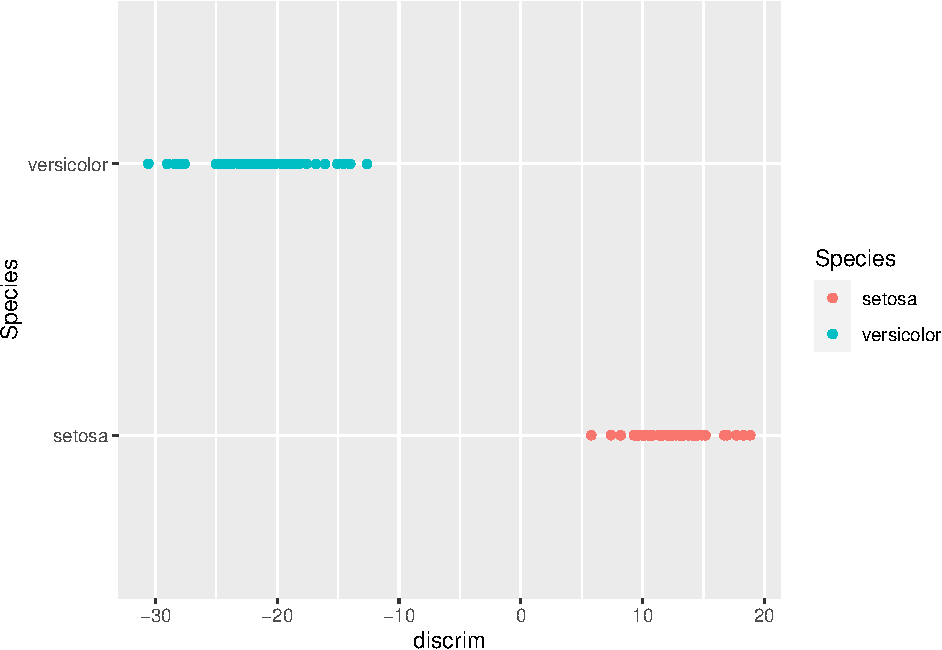
\includegraphics{Homework2_files/figure-latex/unnamed-chunk-4-1.pdf}

Here you can see that our probability quickly converges, especially when
n is large, to .634

\begin{enumerate}
\def\labelenumi{\alph{enumi})}
\setcounter{enumi}{7}
\tightlist
\item
\end{enumerate}

\begin{Shaded}
\begin{Highlighting}[]
\NormalTok{store }\OtherTok{\textless{}{-}} \FunctionTok{rep}\NormalTok{(}\ConstantTok{NA}\NormalTok{, }\DecValTok{10000}\NormalTok{)}
\ControlFlowTok{for}\NormalTok{ (i }\ControlFlowTok{in} \DecValTok{1}\SpecialCharTok{:}\DecValTok{10000}\NormalTok{)\{}
\NormalTok{  store[i] }\OtherTok{\textless{}{-}} \FunctionTok{sum}\NormalTok{(}\FunctionTok{sample}\NormalTok{(}\DecValTok{1}\SpecialCharTok{:}\DecValTok{100}\NormalTok{, }\AttributeTok{rep =} \ConstantTok{TRUE}\NormalTok{) }\SpecialCharTok{==}\DecValTok{4}\NormalTok{)}\SpecialCharTok{\textgreater{}}\DecValTok{0}
\NormalTok{\}}
\FunctionTok{mean}\NormalTok{(store)}
\end{Highlighting}
\end{Shaded}

\begin{verbatim}
## [1] 0.6384
\end{verbatim}

This result makes a lot of sense as the probability of of it being the
4th observation is the same as it being any jth observation, we are just
reaffirming that idea through simulation. This result should and does
fortunately follow the same result as part e!

\hypertarget{simulation-problem-2-code-1.5-pts-explanation-3.5-pts}{%
\subsection{Simulation Problem 2 (Code: 1.5 pts; Explanation: 3.5
pts)}\label{simulation-problem-2-code-1.5-pts-explanation-3.5-pts}}

Copy the \emph{functions} you created in the Bootstrap Confidence
Intervals class activity as well as Simulation Parts 3, 4, and 5.

\begin{Shaded}
\begin{Highlighting}[]
\NormalTok{bootstrap\_resample }\OtherTok{\textless{}{-}} \ControlFlowTok{function}\NormalTok{(data\_vector, B, }\AttributeTok{summary\_fn =}\NormalTok{ mean,}
                               \AttributeTok{seed =} \DecValTok{100}\NormalTok{, ...)\{}
  \CommentTok{\# data\_vector: a vector of data}
  \CommentTok{\# B: the number of bootstrap resamples}
  \CommentTok{\# summary\_fn: the name of a function to apply to the resampled data}
  \CommentTok{\# ...: any additional arguments to summary\_fn}
  
\NormalTok{  boot\_samples }\OtherTok{\textless{}{-}} \FunctionTok{matrix}\NormalTok{(}\DecValTok{0}\NormalTok{, }\AttributeTok{nrow =} \FunctionTok{length}\NormalTok{(data\_vector), }\AttributeTok{ncol =}\NormalTok{ B)}
  
\NormalTok{  n }\OtherTok{\textless{}{-}}\FunctionTok{length}\NormalTok{(data\_vector)}
  \CommentTok{\# We need to add some code here!}
  \FunctionTok{set.seed}\NormalTok{(seed)}
  \ControlFlowTok{for}\NormalTok{ (i }\ControlFlowTok{in} \DecValTok{1}\SpecialCharTok{:}\NormalTok{B) \{}
\NormalTok{     boot\_samples[,i] }\OtherTok{\textless{}{-}} \FunctionTok{sample}\NormalTok{(data\_vector, }\AttributeTok{size =}\NormalTok{ n, }\AttributeTok{replace =} \ConstantTok{TRUE}\NormalTok{)}
    
\NormalTok{  \}}

\NormalTok{  boot\_stat }\OtherTok{\textless{}{-}} \FunctionTok{apply}\NormalTok{(boot\_samples, }\DecValTok{2}\NormalTok{, summary\_fn, ...)}
  \CommentTok{\# Seriously, do not name any arguments x or FUN when using apply within a function}
  \CommentTok{\# Advice from someone who spent 30 minutes debugging a sample solution}
  
  \FunctionTok{return}\NormalTok{(boot\_stat)}
\NormalTok{\}}
\end{Highlighting}
\end{Shaded}

\begin{Shaded}
\begin{Highlighting}[]
\NormalTok{bootstrap\_ci }\OtherTok{\textless{}{-}} \ControlFlowTok{function}\NormalTok{(data\_vector, method, }\AttributeTok{B =} \DecValTok{1000}\NormalTok{, }\AttributeTok{seed =} \DecValTok{100}\NormalTok{, }\AttributeTok{C =} \FloatTok{0.95}\NormalTok{, }\AttributeTok{summary\_fn =}\NormalTok{ mean, ...)\{}
  \CommentTok{\# data\_vector: a vector of data}
  \CommentTok{\# method: the CI method}
  \CommentTok{\# B: the number of bootstrap resamples}
  \CommentTok{\# seed: the seed to use}
  \CommentTok{\# C: the confidence level as a decimal}
  \CommentTok{\# summary\_fn: the name of a function to apply to the resampled data}
  \CommentTok{\# ...: any additional arguments to summary\_fn}


  
\NormalTok{  obs\_stat }\OtherTok{\textless{}{-}} \FunctionTok{do.call}\NormalTok{(summary\_fn, }\AttributeTok{args =} \FunctionTok{list}\NormalTok{(data\_vector, ...))}
  \CommentTok{\# do.call allows you to call a function without having to hard{-}code what that function is}
  \CommentTok{\# the args argument is a list of arguments to the function}
  \CommentTok{\# so this will find the observed value of the statistic given the original data vector}
  
\NormalTok{  bootstrap\_values }\OtherTok{\textless{}{-}} \FunctionTok{bootstrap\_resample}\NormalTok{(data\_vector, B, summary\_fn, ...)}
  
\NormalTok{  alpha }\OtherTok{\textless{}{-}} \DecValTok{1} \SpecialCharTok{{-}}\NormalTok{ C}
  
  \ControlFlowTok{if}\NormalTok{ (method }\SpecialCharTok{==} \StringTok{"percentile"}\NormalTok{)\{}
      \CommentTok{\# write code to get the percentile confidence level out of the returned bootstrap\_values and store in a length 2 vector boot\_ci}
    
\NormalTok{    boot\_ci }\OtherTok{\textless{}{-}} \FunctionTok{quantile}\NormalTok{(bootstrap\_values, }
                        \AttributeTok{probs =} \FunctionTok{c}\NormalTok{(alpha}\SpecialCharTok{/}\DecValTok{2}\NormalTok{, }\DecValTok{1} \SpecialCharTok{{-}}\NormalTok{ alpha}\SpecialCharTok{/}\DecValTok{2}\NormalTok{)}
\NormalTok{                        )}
\NormalTok{  \} }\ControlFlowTok{else} \ControlFlowTok{if}\NormalTok{ (method }\SpecialCharTok{==} \StringTok{"basic"}\NormalTok{)\{}
    \CommentTok{\# write code to get the "basic" confidence level and store in a length 2 vector boot\_ci}
\NormalTok{    boot\_ci }\OtherTok{\textless{}{-}} \DecValTok{2} \SpecialCharTok{*}\NormalTok{ obs\_stat }\SpecialCharTok{{-}} 
      \FunctionTok{quantile}\NormalTok{(bootstrap\_values, }\AttributeTok{probs =} \FunctionTok{c}\NormalTok{(}\DecValTok{1} \SpecialCharTok{{-}}\NormalTok{ alpha}\SpecialCharTok{/}\DecValTok{2}\NormalTok{, alpha}\SpecialCharTok{/}\DecValTok{2}\NormalTok{))}
\NormalTok{  \} }\ControlFlowTok{else} \ControlFlowTok{if}\NormalTok{ (method }\SpecialCharTok{==} \StringTok{"normal"}\NormalTok{)\{}
    \CommentTok{\# write code to get the normal{-}theory confidence interval and store in a length 2 vector boot\_ci}
    \CommentTok{\# make sure to use the adjustments in the course notes, e.g., don\textquotesingle{}t use 1/sqrt(n) as your standard deviation of sample means}
\NormalTok{    center }\OtherTok{\textless{}{-}} \DecValTok{2}\SpecialCharTok{*}\NormalTok{obs\_stat }\SpecialCharTok{{-}} \FunctionTok{mean}\NormalTok{(bootstrap\_values)}
\NormalTok{    crit\_value }\OtherTok{\textless{}{-}} \FunctionTok{qnorm}\NormalTok{(alpha}\SpecialCharTok{/}\DecValTok{2}\NormalTok{)}
\NormalTok{    se\_boot }\OtherTok{\textless{}{-}} \FunctionTok{sd}\NormalTok{(bootstrap\_values)}
\NormalTok{    boot\_ci }\OtherTok{\textless{}{-}}\NormalTok{ center }\SpecialCharTok{+} \FunctionTok{c}\NormalTok{(}\DecValTok{1}\NormalTok{, }\SpecialCharTok{{-}}\DecValTok{1}\NormalTok{) }\SpecialCharTok{*}\NormalTok{ crit\_value }\SpecialCharTok{*}\NormalTok{ se\_boot}
      
\NormalTok{  \}}
  
  \FunctionTok{return}\NormalTok{(boot\_ci)}
\NormalTok{\}}
\end{Highlighting}
\end{Shaded}

\hypertarget{simulation-part-3---assumptions-not-met-large-samples}{%
\subsection{Simulation Part 3 - Assumptions Not Met, Large
Samples}\label{simulation-part-3---assumptions-not-met-large-samples}}

Simulate 1000 sets of 100 random numbers from a \(Exp(1)\) distribution
and store them in a 1000 x 100 matrix \texttt{sim\_data3}. Note that
\texttt{sim\_data3} represents 1000 samples of size 100 under conditions
where we \emph{know} the assumptions of a t confidence interval are not
met but we are hoping that the Central Limit Theorem can cover us.

\begin{Shaded}
\begin{Highlighting}[]
\FunctionTok{set.seed}\NormalTok{(}\DecValTok{437}\NormalTok{)}
\CommentTok{\# need to do the simulation now!}
\NormalTok{sim\_data3 }\OtherTok{\textless{}{-}} \FunctionTok{matrix}\NormalTok{(}\FunctionTok{rexp}\NormalTok{(}\DecValTok{1000}\SpecialCharTok{*}\DecValTok{100}\NormalTok{), }\AttributeTok{nrow =} \DecValTok{1000}\NormalTok{, }\AttributeTok{ncol =} \DecValTok{10}\NormalTok{)}
\end{Highlighting}
\end{Shaded}

\begin{verbatim}
## Warning in matrix(rexp(1000 * 100), nrow = 1000, ncol = 10): data length
## differs from size of matrix: [100000 != 1000 x 10]
\end{verbatim}

Copy and modify your code chunks from Simulation Part 1 to produce 95\%
confidence intervals using \texttt{sim\_data3}. What proportion of
``95\% confidence intervals'' actually contained the true parameter
value? Did any methods perform noticeably better/worse?

\begin{Shaded}
\begin{Highlighting}[]
\CommentTok{\# You should be able to just run this code chunk without any fixes}
\NormalTok{pop\_mean3 }\OtherTok{\textless{}{-}} \DecValTok{1}
\NormalTok{ci\_t3 }\OtherTok{\textless{}{-}} \FunctionTok{apply}\NormalTok{(sim\_data3, }\DecValTok{1}\NormalTok{, }\ControlFlowTok{function}\NormalTok{(x) }\FunctionTok{t.test}\NormalTok{(x)}\SpecialCharTok{$}\NormalTok{conf.int)}
\NormalTok{ci\_t\_df3 }\OtherTok{\textless{}{-}} \FunctionTok{as.data.frame}\NormalTok{(}\FunctionTok{t}\NormalTok{(ci\_t3))}
\FunctionTok{names}\NormalTok{(ci\_t\_df3) }\OtherTok{\textless{}{-}} \FunctionTok{c}\NormalTok{(}\StringTok{"lower"}\NormalTok{, }\StringTok{"upper"}\NormalTok{)}
\NormalTok{ci\_t\_df3 }\SpecialCharTok{\%\textgreater{}\%} \FunctionTok{mutate}\NormalTok{(}\AttributeTok{covered =}\NormalTok{ lower }\SpecialCharTok{\textless{}=}\NormalTok{ pop\_mean3 }\SpecialCharTok{\&}\NormalTok{ upper }\SpecialCharTok{\textgreater{}=}\NormalTok{ pop\_mean3) }\SpecialCharTok{\%\textgreater{}\%}
  \FunctionTok{summarize}\NormalTok{(}\AttributeTok{coverage\_probability =} \FunctionTok{mean}\NormalTok{(covered))}
\end{Highlighting}
\end{Shaded}

\begin{verbatim}
##   coverage_probability
## 1                0.903
\end{verbatim}

\begin{Shaded}
\begin{Highlighting}[]
\CommentTok{\# You should be able to just run this code chunk without any fixes}
\NormalTok{ci\_perc3 }\OtherTok{\textless{}{-}} \FunctionTok{apply}\NormalTok{(sim\_data3, }\DecValTok{1}\NormalTok{, bootstrap\_ci, }\AttributeTok{method =} \StringTok{"percentile"}\NormalTok{, }\AttributeTok{B =} \DecValTok{1000}\NormalTok{, }\AttributeTok{summary\_fn =}\NormalTok{ mean, }\AttributeTok{na.rm =} \ConstantTok{TRUE}\NormalTok{)}
\CommentTok{\# don\textquotesingle{}t need any ... arguments here, but illustrating the idea of the ...}
\CommentTok{\# notice that bootstrap\_ci has default seed = 100 and C = 0.95 arguments}
\NormalTok{ci\_perc\_df3 }\OtherTok{\textless{}{-}} \FunctionTok{as.data.frame}\NormalTok{(}\FunctionTok{t}\NormalTok{(ci\_perc3))}
\FunctionTok{names}\NormalTok{(ci\_perc\_df3) }\OtherTok{\textless{}{-}} \FunctionTok{c}\NormalTok{(}\StringTok{"lower"}\NormalTok{, }\StringTok{"upper"}\NormalTok{)}
\NormalTok{ci\_perc\_df3 }\SpecialCharTok{\%\textgreater{}\%} \FunctionTok{mutate}\NormalTok{(}\AttributeTok{covered =}\NormalTok{ lower }\SpecialCharTok{\textless{}=}\NormalTok{ pop\_mean3 }\SpecialCharTok{\&}\NormalTok{ upper }\SpecialCharTok{\textgreater{}=}\NormalTok{ pop\_mean3) }\SpecialCharTok{\%\textgreater{}\%}
  \FunctionTok{summarize}\NormalTok{(}\AttributeTok{coverage\_probability =} \FunctionTok{mean}\NormalTok{(covered))}
\end{Highlighting}
\end{Shaded}

\begin{verbatim}
##   coverage_probability
## 1                0.857
\end{verbatim}

Copy and modify the chunk above for the basic and normal-theory
intervals.

\begin{Shaded}
\begin{Highlighting}[]
\NormalTok{ci\_basic3 }\OtherTok{\textless{}{-}} \FunctionTok{apply}\NormalTok{(sim\_data3, }\DecValTok{1}\NormalTok{, bootstrap\_ci, }\AttributeTok{method =} \StringTok{"basic"}\NormalTok{, }\AttributeTok{B =} \DecValTok{1000}\NormalTok{, }\AttributeTok{summary\_fn =}\NormalTok{ mean, }\AttributeTok{na.rm =} \ConstantTok{TRUE}\NormalTok{)}

\NormalTok{ci\_basic\_df3 }\OtherTok{\textless{}{-}} \FunctionTok{as.data.frame}\NormalTok{(}\FunctionTok{t}\NormalTok{(ci\_basic3))}
\FunctionTok{names}\NormalTok{(ci\_basic\_df3) }\OtherTok{\textless{}{-}} \FunctionTok{c}\NormalTok{(}\StringTok{"lower"}\NormalTok{, }\StringTok{"upper"}\NormalTok{)}
\NormalTok{ci\_basic\_df3 }\SpecialCharTok{\%\textgreater{}\%} \FunctionTok{mutate}\NormalTok{(}\AttributeTok{covered =}\NormalTok{ lower }\SpecialCharTok{\textless{}=}\NormalTok{ pop\_mean3 }\SpecialCharTok{\&}\NormalTok{ upper }\SpecialCharTok{\textgreater{}=}\NormalTok{ pop\_mean3) }\SpecialCharTok{\%\textgreater{}\%}
  \FunctionTok{summarize}\NormalTok{(}\AttributeTok{coverage\_probability =} \FunctionTok{mean}\NormalTok{(covered))}
\end{Highlighting}
\end{Shaded}

\begin{verbatim}
##   coverage_probability
## 1                0.845
\end{verbatim}

\begin{Shaded}
\begin{Highlighting}[]
\NormalTok{ci\_normal3 }\OtherTok{\textless{}{-}} \FunctionTok{apply}\NormalTok{(sim\_data3, }\DecValTok{1}\NormalTok{, bootstrap\_ci, }\AttributeTok{method =} \StringTok{"normal"}\NormalTok{, }\AttributeTok{B =} \DecValTok{1000}\NormalTok{, }\AttributeTok{summary\_fn =}\NormalTok{ mean, }\AttributeTok{na.rm =} \ConstantTok{TRUE}\NormalTok{)}

\NormalTok{ci\_normal\_df3 }\OtherTok{\textless{}{-}} \FunctionTok{as.data.frame}\NormalTok{(}\FunctionTok{t}\NormalTok{(ci\_normal3))}
\FunctionTok{names}\NormalTok{(ci\_normal\_df3) }\OtherTok{\textless{}{-}} \FunctionTok{c}\NormalTok{(}\StringTok{"lower"}\NormalTok{, }\StringTok{"upper"}\NormalTok{)}
\NormalTok{ci\_normal\_df3 }\SpecialCharTok{\%\textgreater{}\%} \FunctionTok{mutate}\NormalTok{(}\AttributeTok{covered =}\NormalTok{ lower }\SpecialCharTok{\textless{}=}\NormalTok{ pop\_mean3 }\SpecialCharTok{\&}\NormalTok{ upper }\SpecialCharTok{\textgreater{}=}\NormalTok{ pop\_mean3) }\SpecialCharTok{\%\textgreater{}\%}
  \FunctionTok{summarize}\NormalTok{(}\AttributeTok{coverage\_probability =} \FunctionTok{mean}\NormalTok{(covered))}
\end{Highlighting}
\end{Shaded}

\begin{verbatim}
##   coverage_probability
## 1                0.856
\end{verbatim}

\hypertarget{simulation-part-4---assumptions-not-met-small-samples}{%
\subsection{Simulation Part 4 - Assumptions Not Met, Small
Samples}\label{simulation-part-4---assumptions-not-met-small-samples}}

Simulate 1000 sets of 10 random numbers from a \(Exp(1)\) distribution
and store them in a 1000 x 100 matrix \texttt{sim\_data4}. Note that
\texttt{sim\_data4} represents 1000 samples of size 10 under conditions
where we \emph{know} the assumptions of a t confidence interval are not
met and Central Limit Theorem is almost certainly \emph{not} going to
cover us.

\begin{Shaded}
\begin{Highlighting}[]
\FunctionTok{set.seed}\NormalTok{(}\DecValTok{437}\NormalTok{)}
\CommentTok{\# need to do the simulation now!}
\NormalTok{sim\_data4 }\OtherTok{\textless{}{-}} \FunctionTok{matrix}\NormalTok{(}\FunctionTok{rexp}\NormalTok{(}\DecValTok{1000}\SpecialCharTok{*}\DecValTok{10}\NormalTok{), }\AttributeTok{nrow =} \DecValTok{1000}\NormalTok{, }\AttributeTok{ncol =} \DecValTok{10}\NormalTok{)}
\end{Highlighting}
\end{Shaded}

Copy and modify your code chunks from Simulation Part 1 to produce 95\%
confidence intervals using \texttt{sim\_data4}. What proportion of
``95\% confidence intervals'' actually contained the true parameter
value? Did any methods perform noticeably better/worse?

All of the methods performed worse as breaking the central limit theorem
was still an issue even though bootstrapping tends to ignore it. The
range of values was around 84-86\% with the t test being noticeably
better at 90\%.

\begin{Shaded}
\begin{Highlighting}[]
\NormalTok{pop\_mean4 }\OtherTok{\textless{}{-}} \DecValTok{1}
\NormalTok{ci\_t4 }\OtherTok{\textless{}{-}} \FunctionTok{apply}\NormalTok{(sim\_data4, }\DecValTok{1}\NormalTok{, }\ControlFlowTok{function}\NormalTok{(x) }\FunctionTok{t.test}\NormalTok{(x)}\SpecialCharTok{$}\NormalTok{conf.int)}
\NormalTok{ci\_t\_df4 }\OtherTok{\textless{}{-}} \FunctionTok{as.data.frame}\NormalTok{(}\FunctionTok{t}\NormalTok{(ci\_t4))}
\FunctionTok{names}\NormalTok{(ci\_t\_df4) }\OtherTok{\textless{}{-}} \FunctionTok{c}\NormalTok{(}\StringTok{"lower"}\NormalTok{, }\StringTok{"upper"}\NormalTok{)}
\NormalTok{ci\_t\_df4 }\SpecialCharTok{\%\textgreater{}\%} \FunctionTok{mutate}\NormalTok{(}\AttributeTok{covered =}\NormalTok{ lower }\SpecialCharTok{\textless{}=}\NormalTok{ pop\_mean4 }\SpecialCharTok{\&}\NormalTok{ upper }\SpecialCharTok{\textgreater{}=}\NormalTok{ pop\_mean4) }\SpecialCharTok{\%\textgreater{}\%}
  \FunctionTok{summarize}\NormalTok{(}\AttributeTok{coverage\_probability =} \FunctionTok{mean}\NormalTok{(covered))}
\end{Highlighting}
\end{Shaded}

\begin{verbatim}
##   coverage_probability
## 1                0.903
\end{verbatim}

\begin{Shaded}
\begin{Highlighting}[]
\NormalTok{ci\_perc4 }\OtherTok{\textless{}{-}} \FunctionTok{apply}\NormalTok{(sim\_data4, }\DecValTok{1}\NormalTok{, bootstrap\_ci, }\AttributeTok{method =} \StringTok{"percentile"}\NormalTok{, }\AttributeTok{B =} \DecValTok{1000}\NormalTok{, }\AttributeTok{summary\_fn =}\NormalTok{ mean, }\AttributeTok{na.rm =} \ConstantTok{TRUE}\NormalTok{)}
\NormalTok{ci\_perc\_df4 }\OtherTok{\textless{}{-}} \FunctionTok{as.data.frame}\NormalTok{(}\FunctionTok{t}\NormalTok{(ci\_perc4))}
\FunctionTok{names}\NormalTok{(ci\_perc\_df4) }\OtherTok{\textless{}{-}} \FunctionTok{c}\NormalTok{(}\StringTok{"lower"}\NormalTok{, }\StringTok{"upper"}\NormalTok{)}
\NormalTok{ci\_perc\_df4 }\SpecialCharTok{\%\textgreater{}\%} \FunctionTok{mutate}\NormalTok{(}\AttributeTok{covered =}\NormalTok{ lower }\SpecialCharTok{\textless{}=}\NormalTok{ pop\_mean4 }\SpecialCharTok{\&}\NormalTok{ upper }\SpecialCharTok{\textgreater{}=}\NormalTok{ pop\_mean4) }\SpecialCharTok{\%\textgreater{}\%}
  \FunctionTok{summarize}\NormalTok{(}\AttributeTok{coverage\_probability =} \FunctionTok{mean}\NormalTok{(covered))}
\end{Highlighting}
\end{Shaded}

\begin{verbatim}
##   coverage_probability
## 1                0.857
\end{verbatim}

\begin{Shaded}
\begin{Highlighting}[]
\NormalTok{ci\_basic4 }\OtherTok{\textless{}{-}} \FunctionTok{apply}\NormalTok{(sim\_data4, }\DecValTok{1}\NormalTok{, bootstrap\_ci, }\AttributeTok{method =} \StringTok{"basic"}\NormalTok{, }\AttributeTok{B =} \DecValTok{1000}\NormalTok{, }\AttributeTok{summary\_fn =}\NormalTok{ mean, }\AttributeTok{na.rm =} \ConstantTok{TRUE}\NormalTok{)}

\NormalTok{ci\_basic\_df4 }\OtherTok{\textless{}{-}} \FunctionTok{as.data.frame}\NormalTok{(}\FunctionTok{t}\NormalTok{(ci\_basic4))}
\FunctionTok{names}\NormalTok{(ci\_basic\_df4) }\OtherTok{\textless{}{-}} \FunctionTok{c}\NormalTok{(}\StringTok{"lower"}\NormalTok{, }\StringTok{"upper"}\NormalTok{)}
\NormalTok{ci\_basic\_df4 }\SpecialCharTok{\%\textgreater{}\%} \FunctionTok{mutate}\NormalTok{(}\AttributeTok{covered =}\NormalTok{ lower }\SpecialCharTok{\textless{}=}\NormalTok{ pop\_mean4 }\SpecialCharTok{\&}\NormalTok{ upper }\SpecialCharTok{\textgreater{}=}\NormalTok{ pop\_mean4) }\SpecialCharTok{\%\textgreater{}\%}
  \FunctionTok{summarize}\NormalTok{(}\AttributeTok{coverage\_probability =} \FunctionTok{mean}\NormalTok{(covered))}
\end{Highlighting}
\end{Shaded}

\begin{verbatim}
##   coverage_probability
## 1                0.845
\end{verbatim}

\begin{Shaded}
\begin{Highlighting}[]
\NormalTok{ci\_normal4 }\OtherTok{\textless{}{-}} \FunctionTok{apply}\NormalTok{(sim\_data4, }\DecValTok{1}\NormalTok{, bootstrap\_ci, }\AttributeTok{method =} \StringTok{"normal"}\NormalTok{, }\AttributeTok{B =} \DecValTok{1000}\NormalTok{, }\AttributeTok{summary\_fn =}\NormalTok{ mean, }\AttributeTok{na.rm =} \ConstantTok{TRUE}\NormalTok{)}

\NormalTok{ci\_normal\_df4 }\OtherTok{\textless{}{-}} \FunctionTok{as.data.frame}\NormalTok{(}\FunctionTok{t}\NormalTok{(ci\_normal4))}
\FunctionTok{names}\NormalTok{(ci\_normal\_df4) }\OtherTok{\textless{}{-}} \FunctionTok{c}\NormalTok{(}\StringTok{"lower"}\NormalTok{, }\StringTok{"upper"}\NormalTok{)}
\NormalTok{ci\_normal\_df4 }\SpecialCharTok{\%\textgreater{}\%} \FunctionTok{mutate}\NormalTok{(}\AttributeTok{covered =}\NormalTok{ lower }\SpecialCharTok{\textless{}=}\NormalTok{ pop\_mean4 }\SpecialCharTok{\&}\NormalTok{ upper }\SpecialCharTok{\textgreater{}=}\NormalTok{ pop\_mean4) }\SpecialCharTok{\%\textgreater{}\%}
  \FunctionTok{summarize}\NormalTok{(}\AttributeTok{coverage\_probability =} \FunctionTok{mean}\NormalTok{(covered))}
\end{Highlighting}
\end{Shaded}

\begin{verbatim}
##   coverage_probability
## 1                0.856
\end{verbatim}

\hypertarget{simulation-part-5---range-preservation}{%
\subsection{Simulation Part 5 - Range
Preservation}\label{simulation-part-5---range-preservation}}

Produce a histogram of the lower bound of the CIs you obtained using
each of the four methods in Simulation Part 4. Which methods appear to
be range-preserving (that is, cannot give implausible values for the
parameter) even under this ``worst-case scenario''?

\begin{Shaded}
\begin{Highlighting}[]
\FunctionTok{par}\NormalTok{(}\AttributeTok{mfrow=} \FunctionTok{c}\NormalTok{(}\DecValTok{2}\NormalTok{,}\DecValTok{2}\NormalTok{))}
\FunctionTok{hist}\NormalTok{(ci\_normal\_df4}\SpecialCharTok{$}\NormalTok{lower)}
\FunctionTok{hist}\NormalTok{(ci\_basic\_df4}\SpecialCharTok{$}\NormalTok{lower)}
\FunctionTok{hist}\NormalTok{(ci\_perc\_df4}\SpecialCharTok{$}\NormalTok{lower)}
\FunctionTok{hist}\NormalTok{(ci\_t\_df4}\SpecialCharTok{$}\NormalTok{lower)}
\end{Highlighting}
\end{Shaded}

\includegraphics{Homework2_files/figure-latex/unnamed-chunk-6-1.pdf}

Write a brief summary of what you learned from the activity. Make sure
to address the following questions:

\begin{itemize}
\tightlist
\item
  Are theory-based methods \emph{guaranteed} to achieve the appropriate
  coverage? What about bootstrap-based methods?
\item
  Which of the four methods appear to be range-preserving even in a
  ``worst-case scenario''?
\item
  When and why would a bootstrap method be useful to obtain a confidence
  interval even if it doesn't achieve the appropriate coverage?
\end{itemize}

\end{document}
